\section{Обзор существующих решений}

Для решения поставленных задач нужен системный подход. Множество компаний и исследовательских групп предлагают различные решения как аппаратной части, так и программной.
 
Компания \textit{Rethink Robotics}, известная своими манипуляторами Sawyer и Baxter~\cite{baxter} для работы на заводах совместно с людьми. Робот Baxter представлен на рисунке~\ref{img:baxter}.

\begin{figure}[h!]
	\centering{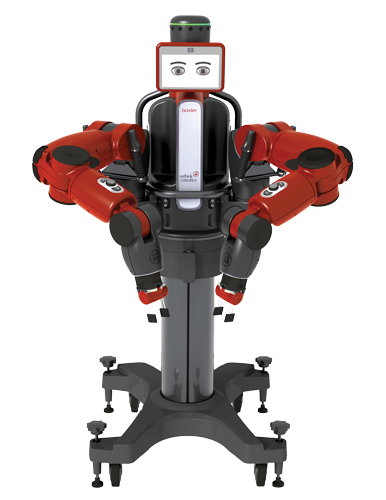
\includegraphics[width=0.4\linewidth]{baxter1.png}}
	\caption{Робот Baxter}
	\label{img:baxter}
\end{figure}

Отличительной особенностью этих роботов является изменение их конфигурации под нужные технологические процессы происходит в виде <<обучения>> в специальном графическом приложении Intera Studio~\ref{img:intera}, а не классического программирования промышленных роботов. Особенностью технологий Rethink Robotics являются роботы, которые экономически эффективны и могут работать совместно с коллегами-людьми, выполняя, например, опасные для людей работы. 

\begin{figure}[h!]
	\centering{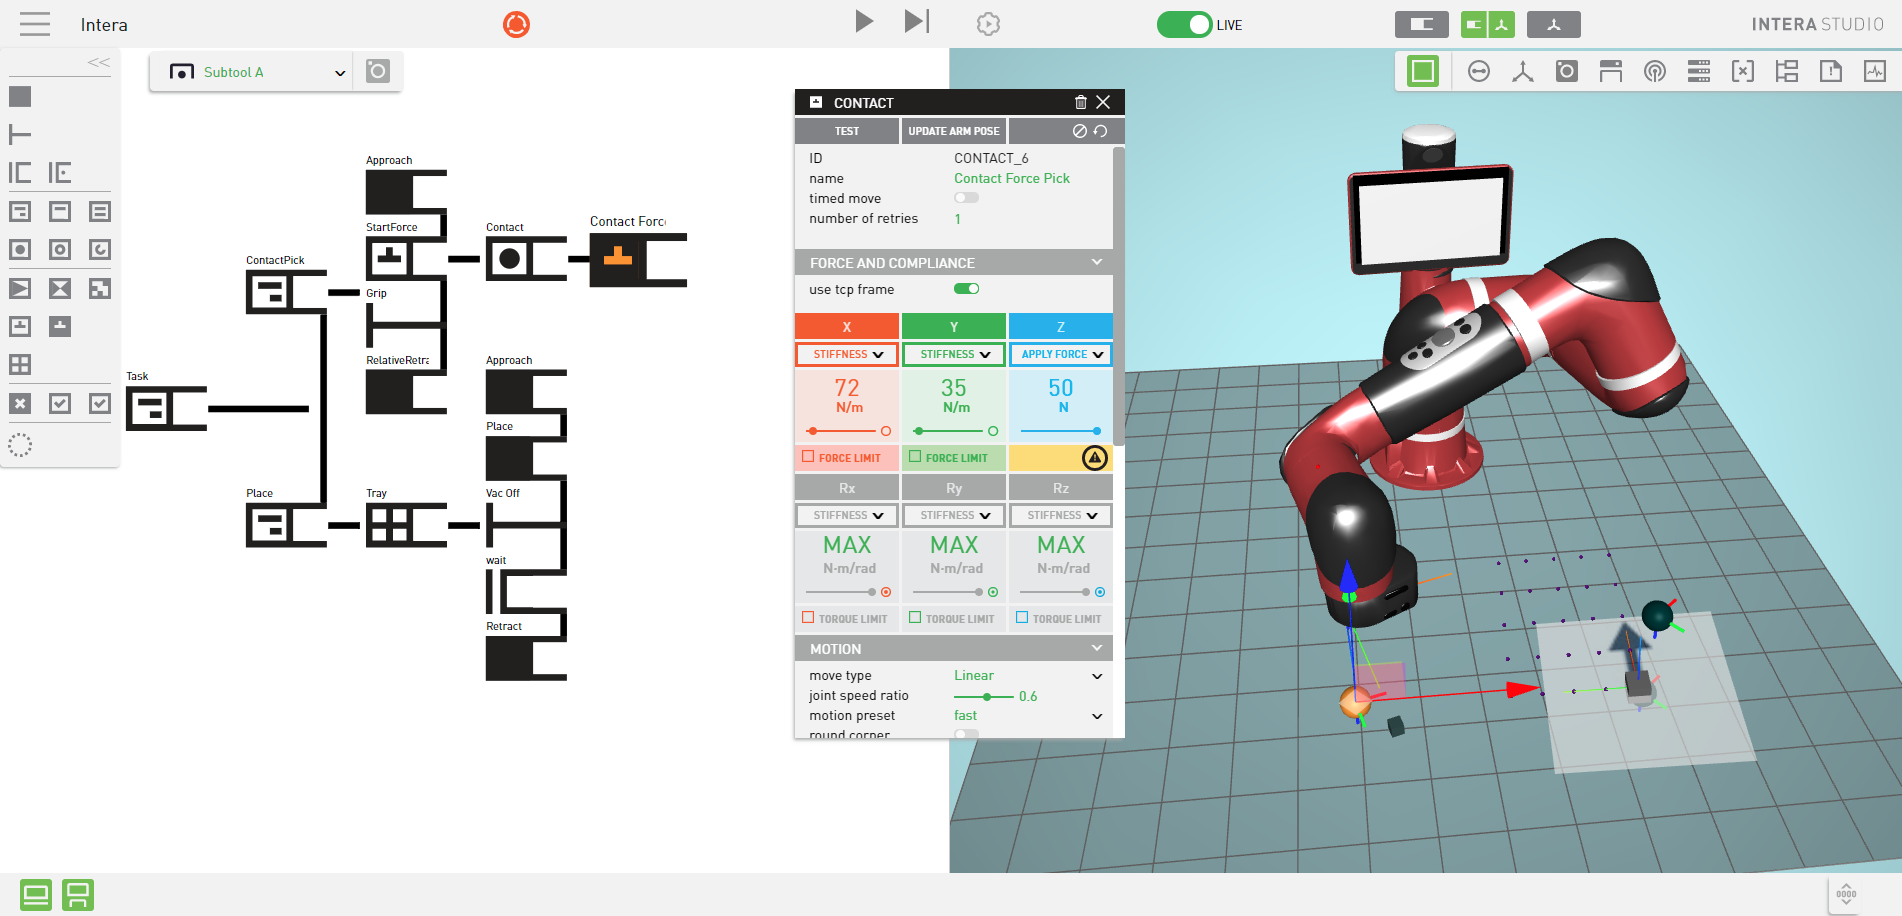
\includegraphics[width=1\linewidth]{intera.png}}
	\caption{Окно приложения Intera Studio для программирования роботов компании Rethink Robotics}
	\label{img:intera}
\end{figure}

По периметру <<головы>> робота располагаются датчики, которые дают возможность ему адаптироваться к окружающей среде, определять наличие людей рядом. В <<руках>> робота установлены инфракрасные датчики. Доступно большое разнообразие схватов.

Многие университеты используют робота Baxter в рамках своих курсов по робототехнике~\cite{baxteruse}, чтобы дать студентам возможность использования современной технологии робототехники для практического применения в реальном мире. Baxter, в отличие от традиционных роботов-манипуляторов, не требует установки вокруг себя заграждений, поэтому студенты могут работать с ним в непосредственной близости, не беспокоясь о безопасности.
% http://www.rethinkrobotics.com/

%%%%%%%%%%%%%%%%%%%%
%%% Robotnik RB-1
\textit{Robotnik}~--- испанская компания, специализирующаяся на разработке роботов и R\&D в области робототехники. Один из их роботов RB-1, это модульный мобильный манипулятор, разработанный с возможностью расширения. Применяется  для R\&D, AAL (Ambient Assisted Living) и удаленного управления. Изображение робота показано на рисунке~\ref{img:rb1}.

\begin{figure}[h!]
	\centering{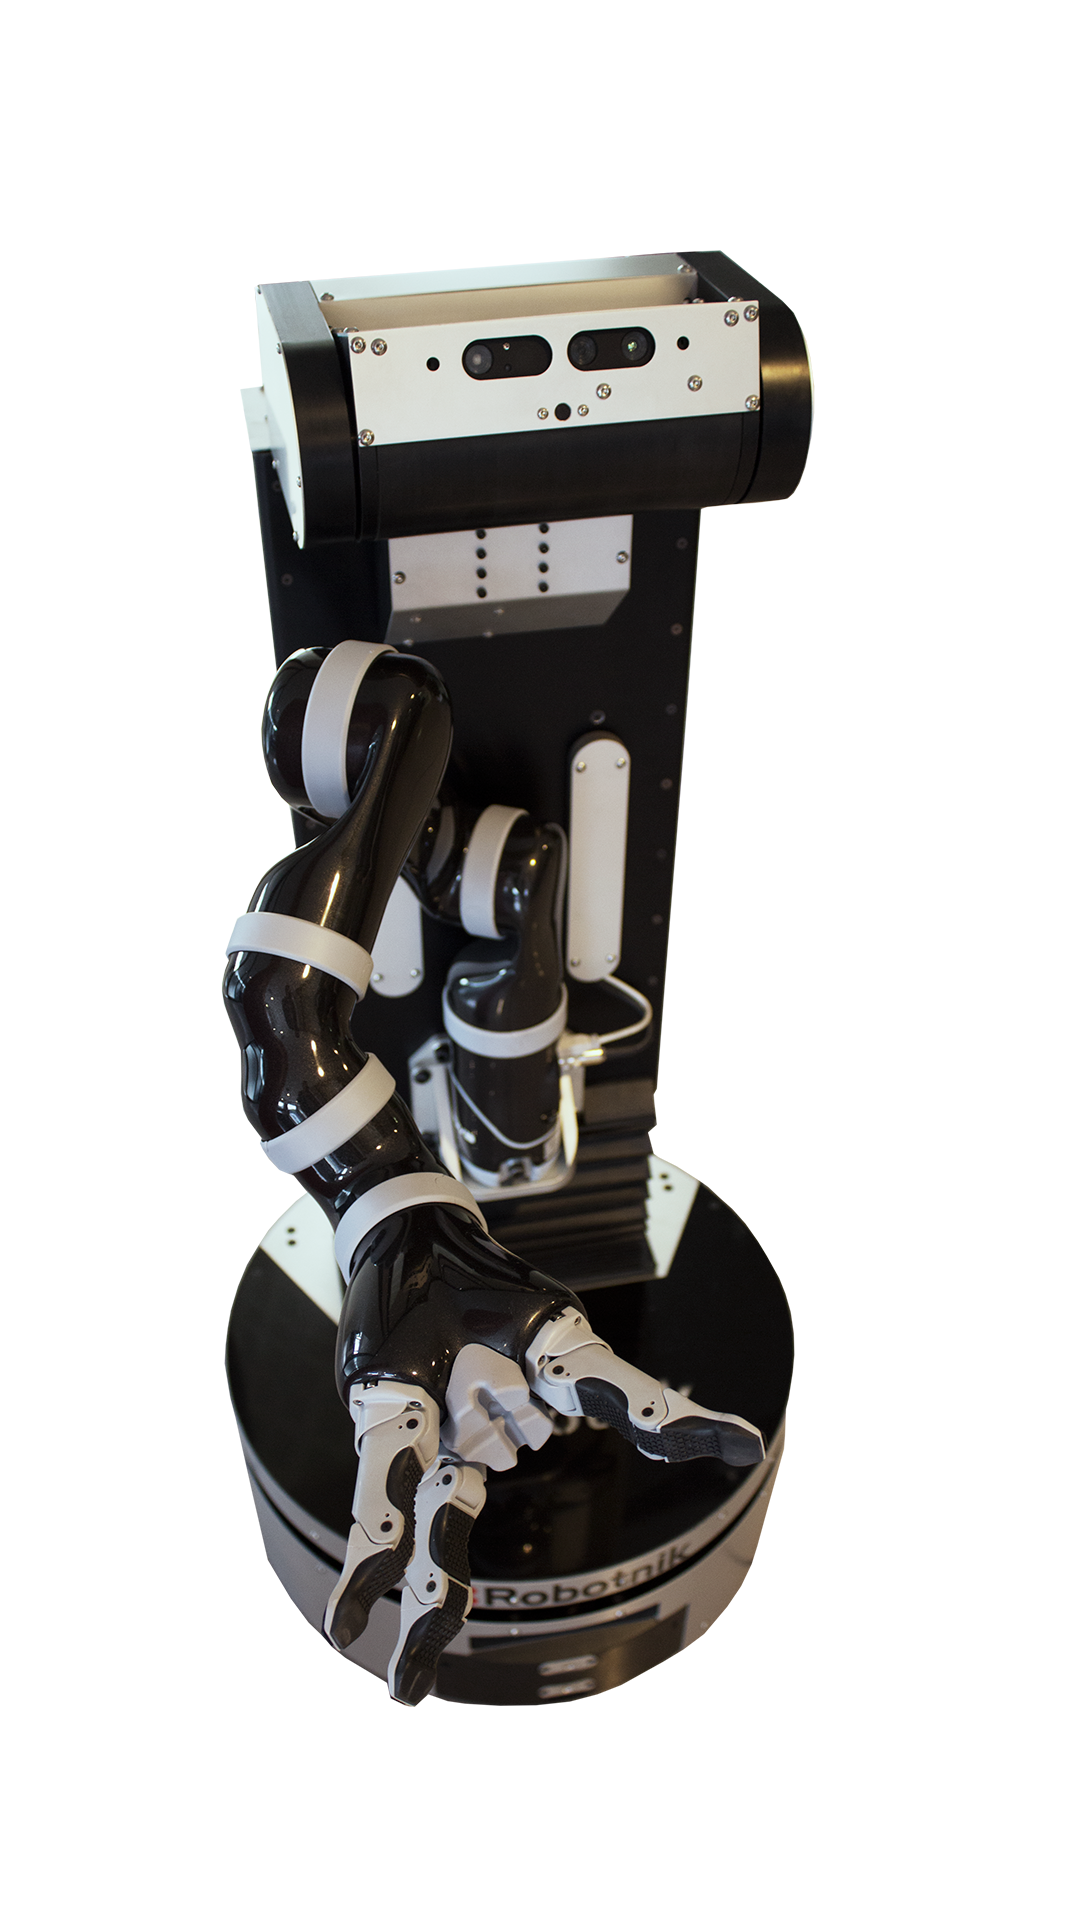
\includegraphics[width=0.30\linewidth]{rb1.png}}
	\caption{Робот испанской компании Robotnik RB-1}
	\label{img:rb1}
\end{figure}

Манипулятор имеет антропоморфную конфигурацию с семью степенями свободы и двух или трехпальцевый захват. Что касается датчиков, в мобильной платформе RB-1 установлен лидар Hokuyo URG-04LX-UG01, для задач навигации и система компьютерного зрения с одной из RGBD камер Microsoft Kinect или  ASUS Xtion PRO Live.

Программное обеспечения с открытыми исходными кодами, управление реализуется посредством ROS (Robotic Operation System). Компания поставляет роботов в нескольких модификациях~\cite{review}.
% https://www.robotnik.eu/manipulators/rb-one/


%%%%%%%%%%%%%%%%%%%%
%%% PAL Robotics TIAGO 
\textit{PAL Robotics}~--- испанская команда вдохновленных инженеров, которые разрабатывают, изготавливают и модифицируют роботов. Их робот TIAGo (Take It And Go)~--- мобильная исследовательская платформа, предназначенная для навигации, манипуляции и взаимодействия с окружающим миром. Оснащена дифференциальной платформой. 

Робот включает в себя систему технического зрения, подъемный торс и манипулятор, обеспечивающие большое рабочее пространство. Полностью совместим с ROS и, кроме того, поставляется с множеством готовых функциональных возможностей, таких как: мультисенсорная навигация, планирование движения без конфликтов, обнаружение людей, лиц и объектов, распознавание речи и синтез. Общий вид робота представлен на рисунке~\ref{img:tiago}~\cite{review}.

\begin{figure}[h!]
	\centering{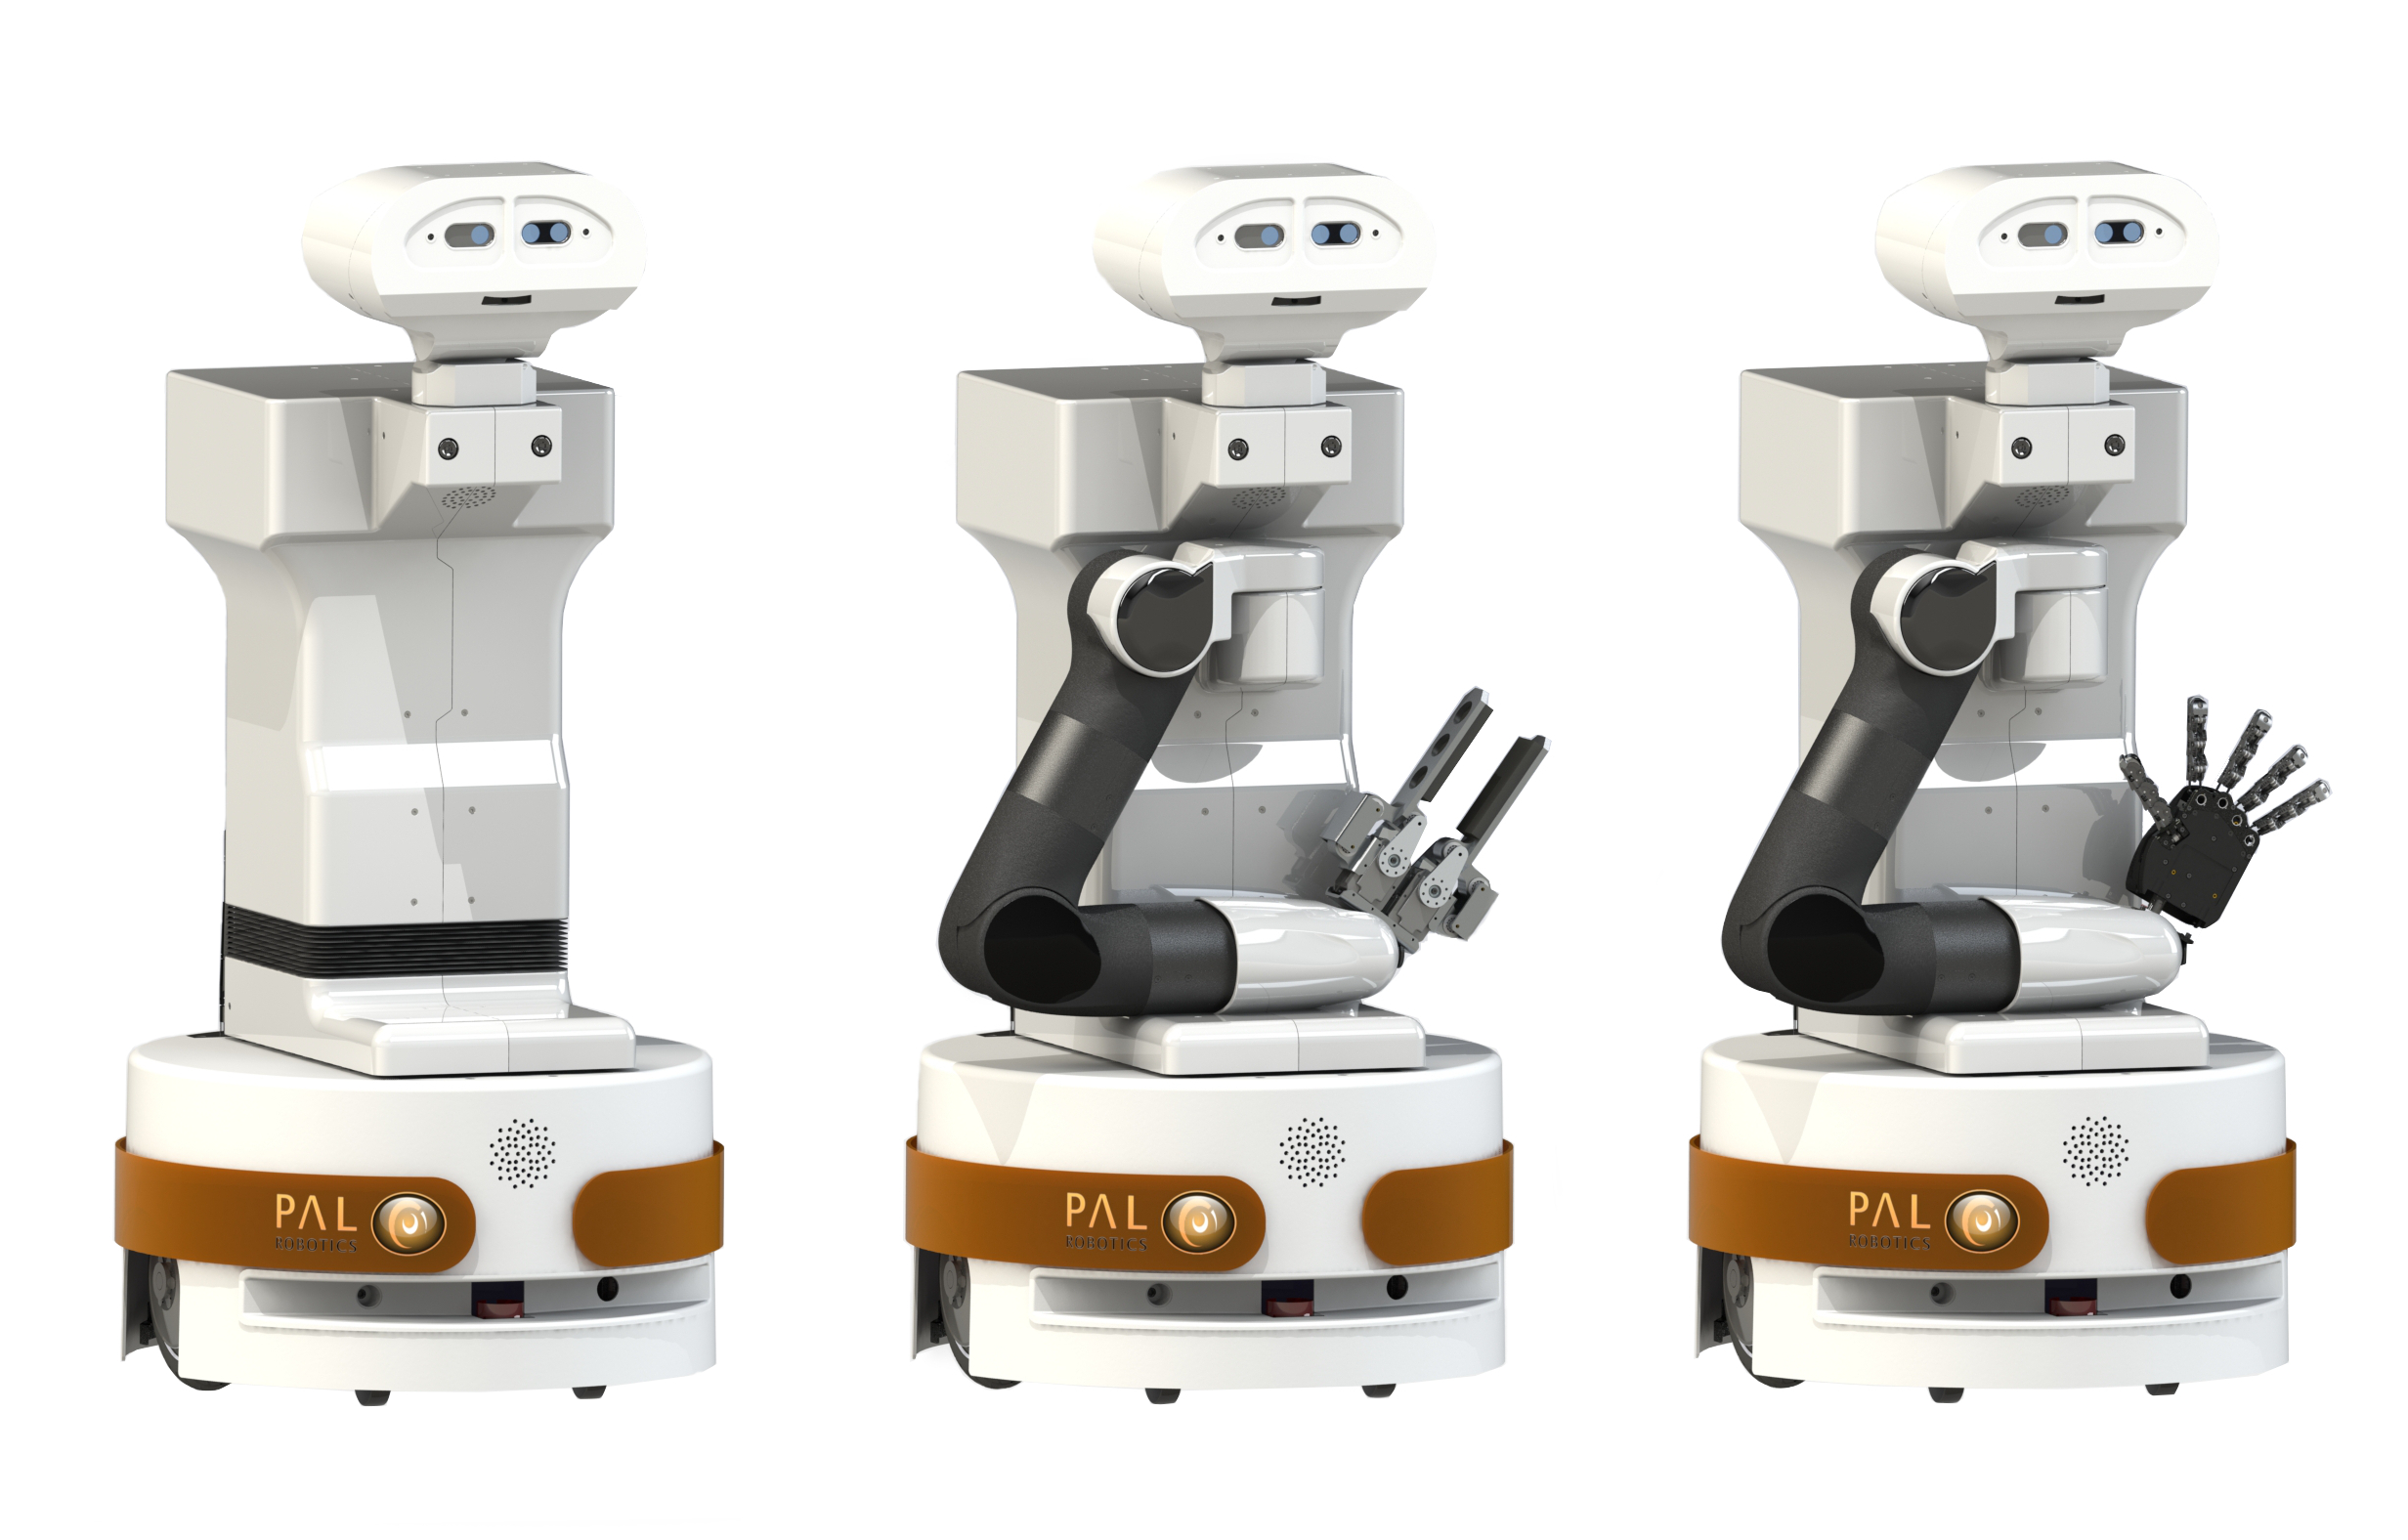
\includegraphics[width=0.9\linewidth]{tiago.jpg}}
	\caption{Робот испанской компании PAL Robotics TIAGO}
	\label{img:tiago}
\end{figure}


%%%%%%%%%%%%%%%%%%%%
%%% Care-O-bot 4 
\textit{Fraunhofer IPA}~--- немецкая компания, выпускающая целую линейку роботов, для исследований. Один из них Care-O-bot 4, изображение которого представлено на рисунке~\ref{img:careobot}.

\begin{figure}[h!]
	\centering{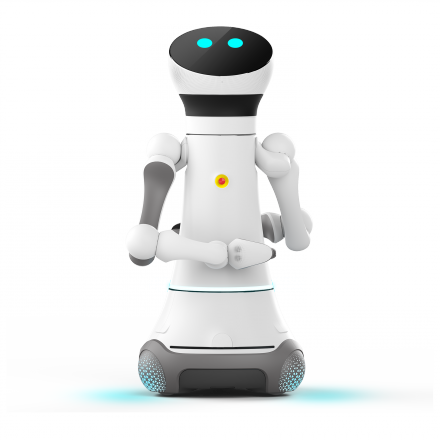
\includegraphics[width=0.5\linewidth]{careobot.png}}
	\caption{Робот немецкой компании Fraunhofer IPA Care-O-bot 4}
	\label{img:careobot}
\end{figure}

Самое интересное в Care-O-bot 4 (кроме двух рук и изысканных движений)~--- его модульность. Робот состоит из пяти модулей: основание, туловище, руки, кольцо датчиков и голова. Каждый из модулей может быть отсоединён, в зависимости от задач.

Робот может найти применение как дома, в качестве повседневного помощника, так и в муниципальных учреждениях для оказания различных услуг~\cite{review}.
% http://www.mojin-robotics.de/

\textit{Moley Robotics}~--- это робототехническая компания, основанная Марком Олейник в 2015 году для создания сервисных роботов для использования на кухне. Прототип робота Moley Robotic Kitchen~--- это роботизированная кухня. Изображение прототипа показано на рисунке~\ref{img:moley}

\begin{figure}[h!]
	\centering{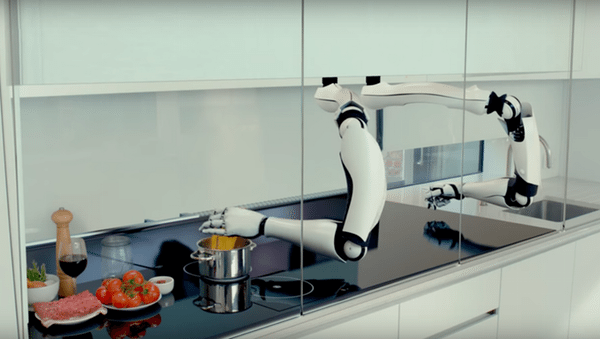
\includegraphics[width=0.9\linewidth]{moley2.png}}
	\caption{Робот компании Moley Robotic Kitchen}
	\label{img:moley}
\end{figure}

Moley Robotic Kitchen включает в себя два манипулятора со схватами в виде кистей рук, оснащенные тактильными датчиками, кухонный стол с духовкой, электрической плитой, посудомоечной машиной и сенсорным экраном. Манипуляторы могут захватывать и взаимодействовать с большинством кухонных принадлежностей~\cite{moley}.

Робот умеет запоминать движения человека, когда тот готовит некоторое блюдо и затем, воспроизводить их при приготовлении того же блюда самостоятельно.

В текущем прототипе пользователь управляет установкой с помощью встроенного сенсорного экрана или приложения для смартфона с готовыми ингредиентами, приготовленными заранее и помещенными в определенные места. Целью Moley Robotic в будущем является предоставление пользователю возможности выбирать из библиотеки более 2000 записанных рецептов.

Исследовательский робот немецкой компании \textit{KUKA} YouBot~--- образовательный робот, специально разработанный для разработки и обучения в области мобильных манипуляторов. Он состоит из омни-платформы, пятистепенного манипулятора и двухпальцевого схвата. KUKA YouBot~--- это платформа с открытым исходным кодом, представлена на рисунке~\ref{img:ky}.

\begin{figure}[h!]
	\centering{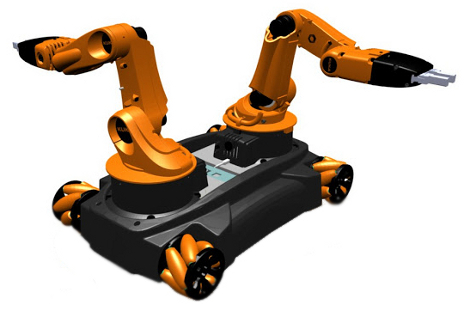
\includegraphics[width=0.8\linewidth]{ky.jpg}}
	\caption{Робот компании KUKA YouBot}
	\label{img:ky}
\end{figure}

\newpage